Comme vu précédemment, l'algorithme High Label analyse les n\oe uds en fonction de la valeur de leur
fonction de distance. Cette sélection permet d'obtenir une borne maximale en $O(n^2\sqrt{m})$, c'est
ce que nous allons démontrer.

Soit une constante $K = \sqrt{m}$, soit la fonction $d': S \longrightarrow \mathbb{N}$, définie par
: $$
d'(i) = |\{j : d(j) \leq d(i) \}| \quad \forall i,j \in S $$
Autrement dit, $d'(i)$ représente le nombre de n\oe uds de $S$ étant plus proche du puits que $i$.
Cette fonctions vérifie alors quelques propriétés : 
\begin{lemma}
	$$\forall i \in S, \quad d'(i) \leq n$$
\end{lemma}

\underline{\textbf{Preuve :}}\\
L'ensemble des sommets dont la distance est inférieure à une valeur donnée est un sous-ensemble de
l'ensemble des sommets du graphe. Son cardinal est donc majoré par ce dernier.
Introduisons la fonction de potentiel $\Phi$ définie comme suit : $$
\Phi = \sum_{i : e(i) > 0} d'(i) / K $$

On peut remarquer qu'à n'importe quel moment de l'exécution de l'algorithme, $\Phi \geq 0$ et que
après l'initialisation : $Phi \leq n^2 / K$. Cette borne est atteinte dans le cas d'un graphe
complet puisque chaque n\oe ud ayant une distance de 1 et étant relié à la source, on obtient alors
$n$ n\oe uds actifs vérifiant tous $d'(n) = n$, d'où $\Phi = n^2/K$.

Regardons les effets des opérations de poussage et réétiquetage sur la fonction $\Phi$.

\begin{lemma}
	Une opération de réétiquetage augmente la valeur de $\Phi$ d'au plus $n/K$.
\end{lemma}

\underline{\textbf{Preuve :}}\\Dans le pire des cas, le sommet réétiqueté passe de la plus petite
distance du graphe à la plus grande. Une représentation d'un de ces cas est donnée \ref{pdc}. Il
s'agit là d'une chaîne dont la capacité de chacun des arcs est supérieure à la capacité du dernier
arc de la chaîne, de façon à ce que l'on observe un phénomène de flux et reflux influant sur la
distance de tous les sommets. Lors du dernier réétiquetage de l'algorithme on se retrouve dans le
cas représenté.
Aucun autre n\oe ud n'étant actif, on a, avant réétiquetage, $\Phi = d'(1) / K = 1/K$, or après
réétiquetage, le sommet $1$ est le sommet présentant la plus haute distance du graphe. On observe
dans ce cas une augmentation de $k/K$ soit $(n-2)/k$.

\begin{figure}
	\begin{center}
		\subfloat[Le graphe de flots]{
			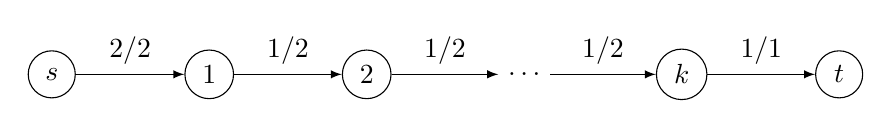
\begin{tikzpicture}
				\tikzset{n/.style={draw=black, circle, minimum size=17pt},f/.style={->,>=latex}};
				\node[n] (s) at (0,0) {$s$};
				\node[n] (1) at (2,0) {$1$};
				\node[n] (2) at (4,0) {$2$};
				\node (pt) at (6,0) {$\dots$};
				\node[n] (k) at (8,0) {$k$};
				\node[n] (t) at (10,0) {$t$};

				\draw[f] (s) to node[above] {$2/2$}(1) ;
				\draw[f] (1) to node[above] {$1/2$}(2) ;
				\draw[f] (2) to node[above]  {$1/2$}(pt);
				\draw[f] (pt) to node[above] {$1/2$} (k);
				\draw[f] (k) to node[above] {$1/1$}(t) ;
			\end{tikzpicture}}
		\subfloat[Excédents, distances et fonctions de potentiel]{
			\begin{tabular}{|c|c|c|c|} \hline
				$i$ & $d(i)$ & $e(i)$ & $d'(i)$ \\ \hline
				$s$ & $k+2$ & $\infty$ & $k+1$ \\ \hline
				$1$ & $k+1$ & $1$ & $1$ \\ \hline
				$2$ & $k+2$ & $0$ & $n+1$ \\ \hline
				$\dots$ & $\dots$ & $\dots$ & $\dots$ \\ \hline
				$n$ & $k+2$ & $0$ & $k+1$ \\ \hline
				$t$ & $0$ & $1$ & $0$ \\ \hline
				& & & $\Phi = 1/K$ \\ \hline
			\end{tabular}}
	\end{center}
	\label{pdc}
	\caption{Exemple de l'influence du réétiquetage sur la fonction $\Phi$}
\end{figure}

\begin{lemma}
	Une opération de poussage saturant augmente la valeur de $\Phi$ d'au plus $n/K$.
\end{lemma}

\underline{\textbf{Preuve :}}\\
Chaque opération de poussage non saturant rend actif, au plus un seul sommet supplémentaire,
appelons $k$ ce sommet. Or on sait que $d'(k) \leq n$, donc l'augmentation de $\Phi$ par l'ajout
d'un sommet actif est bornée par $n/K$.

\begin{lemma}
	Une opération de poussage non saturant n'augmente pas la valeur de $\Phi$.
\end{lemma}

\underline{\textbf{Preuve :}}\\
Soient $i$ et $j$ deux sommets tels qu'il est possible de réaliser un poussage non saturant de $i$
vers $j$.  Après cette opération, le sommet $i$ n'est plus actif et le sommet $j$ le devient, or
$d(i) = d(j) + 1$ donc $d'(i) > d'(j)$, on observe même une diminution de la valeur de $\Phi$ d'au
moins $1/K$.

Afin de quantifier le nombre de poussage non saturant, l'algorithme est scindée en phases définie
comme suit : une phase est l'ensemble des opérations de poussage ayant lieu entre deux changements
consécutifs de la valeur :
\begin{equation}
	d^* = \max\{d(v) : v \mbox{ est actif }\}
\end{equation}

Autrement dit il s'agit de l'ensemble des poussages ayant lieu sans qu'il y ait changement de la
valeur maximale des distances des n\oe uds.
Une phase présentant un nombre d'opérations de poussage non saturant supérieure à $K$ sera dite
\emph{faible}, elle sera désignée comme \emph{forte} sinon.

\begin{lemma}
	Le nombre de phases est inférieur à $4n^2$
\end{lemma}

\underline{\textbf{Preuve :}}\\
Au début et à la fin de l'algorithme, $d^* = 0$ dans la mesure où il n'existe aucun sommet actif
dans le graphe. De plus la seule opération capable d'augmenter la valeur de $d^*$ est un
réétiquetage. Puisque $d^*$ augmente au plus de $2n^2$\footnote{Cette borne provient du nombre maximal
de réétiquetage}, sa valeur diminue au plus $2n^2$, on a alors au plus $4n^2$ changements, donc
autant de phases.

\begin{corol}
	Le nombre maximum de poussages non saturants en phase \emph{faible} est borné par $4n^2K$.
\end{corol}

Cecii est directement donné par la limite du nombre de phases : à supposer que toutes les phases
sont des phases faibles, présentant au plus $K$ poussages non saturants. Il y a alors, au maximum,
$4n²K$ poussages non saturants sur l'ensemble de l'algorithme.

\begin{lemma}
	Une phase forte présentant $Q>K$ poussages non saturant diminue la valeur de $\Phi$ d'au moins
	$Q$.
\end{lemma}

\underline{\textbf{Preuve :}}\\
Considérons un phase forte au cours de laquelle sont effectuées $Q$ poussages non saturant.
Dans la mesure où chacune de ces opération a lieu dans la même phase, la valeur de $d^*$ est
constante, ce qui implique que chacune de ces opérations est faite depuis un n\oe ud $i$ tel que
$d(i) = d^*$.

La phase s'achève lorsque, tous les sommets de distance $d^*$ sont sortis de leur état actif, ou
lorsque l'un d'entre eux est réétiqueter impliquant une nouvelle valeur de $d^*$. Dans les deux cas,
puisqu'il s'agit d'une phase forte, il y a au moins $Q$ n\oe uds, qui ont vu leur excédent chuter à
zéro, réduisant ainsi la valeur de $\Phi$ d'au moins $Q/K$ à chaque poussage non
saturant\footnote{Ceci est dû au fait qu'il y a au moins $Q$ n\oe ud ayant la même distance que le
sommet effectuant le poussage. Si l'on appelle $i$ ce sommet $d'(i) \geq Q$}. Or $Q>K$
donc chaque poussage diminue $\Phi$ d'au moins $1$ et donc la phase diminue $\Phi$ d'au moins $Q$.

\begin{theorem}
	L'algorithme High Label s'exécute en $O(n²\sqrt{m})$.
\end{theorem}

L'augmentation maximale de la fonction de potentielle $\Phi$ est égale à $(2n²+2nm)n/K$\footnote{Il
	y a au plus $An²$ réétiquetage et $2nm$ poussages saturant augmentant la valeur de $\Phi$ d'au
plus $n/K$}. Donc la valeur maximale de $\Phi$ se résume à sa valeur initiale maximale ($n²/K$) à
laquelle est ajoutée l'augmentation maximale $(2n²+2nm)n/K$, on obtient alors : $$
\Phi_{\max} = \frac{2n³ + n² + 2n²m}{K} $$

De plus, par définition du principe de fonction potentielle
